\documentclass[aspectratio=169, table]{beamer}
\usepackage[utf8]{inputenc}
\usepackage{listings} 
\usepackage[strings]{underscore}
\usepackage{caption}
\usepackage{float}

\usepackage{tikz}
\usetikzlibrary{shapes.geometric, arrows.meta, trees, positioning}


\renewcommand{\lstlistingname}{} 

\makeatletter
\def\input@path{{../../themes/Pradita}}
\makeatother

\usetheme{Pradita}

\subtitle{IF120203-Programming Fundamentals}

\title{Chapter-08:\\\LARGE{Exception\\}
\vspace{10pt}}
\date[Serial]{\scriptsize {PRU/SPMI/FR-BM-18/0222}}
\author[Pradita]{\small{\textbf{Alfa Yohannis}}}


% Define Python language style for listings
\lstdefinestyle{PythonStyle}{
    language=Python,
    basicstyle=\ttfamily\footnotesize,
    keywordstyle=\color{blue}\bfseries,
    commentstyle=\color{gray}\itshape,
    stringstyle=\color{red},
    showstringspaces=false,
    breaklines=true,
    frame=lines,
    numbers=left,
    numberstyle=\tiny\color{gray},
    backgroundcolor=\color{lightgray!10},
    tabsize=2,
    captionpos=b
}

\lstdefinelanguage{bash} {
	keywords={},
	basicstyle=\ttfamily\small,
	keywordstyle=\color{blue}\bfseries,
	ndkeywords={iex},
	ndkeywordstyle=\color{purple}\bfseries,
	sensitive=true,
	commentstyle=\color{gray},
	stringstyle=\color{red},
	numbers=left,
	numberstyle=\tiny\color{gray},
	breaklines=true,
	frame=lines,
	backgroundcolor=\color{lightgray!10},
	tabsize=2,
	comment=[l]{\#},
	morecomment=[s]{/*}{*/},
	commentstyle=\color{gray}\ttfamily,
	stringstyle=\color{purple}\ttfamily,
	showstringspaces=false,
	captionpos=b
}

\begin{document}

\frame{\titlepage}

% Add table of contents slide
\begin{frame}[fragile]{Contents}
\vspace{15pt}
\begin{columns}[t]
\begin{column}{.4\textwidth}
\tableofcontents[sections={1-4}]
\end{column}
\begin{column}{.6\textwidth}
\tableofcontents[sections={5-7}]
\end{column}
\end{columns}
\end{frame}


\section{Pendahuluan}
\begin{frame}[fragile]{Pendahuluan}
\vspace*{20pt}
\begin{itemize}
  \item Error tak terhindarkan; bagian penting dari proses belajar.
  \item Dua jenis: \textbf{syntax error} (sebelum eksekusi) vs \textbf{runtime error}/\textbf{exception} (saat berjalan).
  \item \texttt{try-except} mencegah program berhenti mendadak.
  \item \texttt{else} untuk alur normal; \texttt{finally} untuk \emph{cleanup}.
  \item \emph{Custom exception} mengekspresikan aturan domain.
  \item Tujuan: program \emph{robust}, informatif saat error, mudah dirawat.
\end{itemize}
\end{frame}

\section{Konsep Dasar Exception}

\begin{frame}[fragile]{Konsep Dasar Exception}
\vspace*{20pt}
\begin{itemize}
  \item Kesalahan (\textit{error}) menyebabkan program tidak berjalan sebagaimana mestinya.
  \item Python menyediakan mekanisme sistematis untuk menangani kesalahan.
  \item Dua kategori utama:
    \begin{itemize}
        \item \textbf{Syntax Error} – kesalahan penulisan kode.
        \item \textbf{Runtime Error / Exception} – kesalahan saat program dijalankan.
    \end{itemize}
  \item \textbf{Exception} memungkinkan program tetap berjalan dengan aman.
\end{itemize}
\end{frame}

% ----------------------------------------------------------
\subsection*{Kesalahan Sintaks (Syntax Error)}
\begin{frame}[fragile]{Kesalahan Sintaks (Syntax Error)}
\vspace*{20pt}
\begin{itemize}
  \item Terjadi ketika kode tidak mengikuti aturan bahasa Python.
  \item Diketahui sebelum program dijalankan.
\end{itemize}

\begin{lstlisting}[style=PythonStyle]
# Contoh kesalahan sintaks: tanda kurung kurang
print("Halo dunia"
\end{lstlisting}

\begin{lstlisting}[language=bash]
SyntaxError: unexpected EOF while parsing
\end{lstlisting}

\begin{itemize}
  \item Interpreter mendeteksi akhir baris yang tidak sesuai,
  biasanya karena tanda kurung penutup hilang.
\end{itemize}
\end{frame}

% ----------------------------------------------------------
\subsection*{Kesalahan Saat Berjalan (Runtime Error)}
\begin{frame}[fragile]{Kesalahan Saat Berjalan (Runtime Error)}
\vspace*{20pt}
\begin{itemize}
  \item Terjadi saat eksekusi program berlangsung.
  \item Kode benar secara sintaks, tetapi gagal ketika dijalankan.
\end{itemize}

\begin{lstlisting}[style=PythonStyle]
# Contoh kesalahan runtime: pembagian dengan nol
hasil = 10 / 0
print(hasil)
\end{lstlisting}

\begin{lstlisting}[language=bash]
ZeroDivisionError: division by zero
\end{lstlisting}

\begin{itemize}
  \item Kesalahan ini disebut \textbf{exception}.
  \item Dapat ditangani agar program tetap berjalan.
\end{itemize}
\end{frame}

% ----------------------------------------------------------
\subsection*{Apa Itu Exception?}
\begin{frame}[fragile]{Apa Itu Exception?}
\vspace*{20pt}
\begin{itemize}
  \item \textbf{Exception} adalah peristiwa saat program berjalan
  yang mengganggu alur normal eksekusi.
  \item Beberapa contoh exception bawaan Python:
  \begin{itemize}
    \item \texttt{ZeroDivisionError} – pembagian dengan nol.
    \item \texttt{IndexError} – akses indeks list di luar jangkauan.
    \item \texttt{ValueError} – tipe atau nilai data tidak valid.
    \item \texttt{FileNotFoundError} – file tidak ditemukan.
    \item \texttt{TypeError} – operasi pada tipe data yang salah.
  \end{itemize}
\end{itemize}

\begin{lstlisting}[style=PythonStyle]
# Beberapa contoh exception umum
angka = [1, 2, 3]
print(angka[5])     # IndexError
int("abc")          # ValueError
with open("data.txt") as f:  # FileNotFoundError
    isi = f.read()
\end{lstlisting}
\end{frame}

\begin{frame}[fragile]{Mengapa Perlu Menangani Exception}
\vspace*{20pt}
\begin{itemize}
  \item Tanpa penanganan exception, kesalahan akan langsung menghentikan program.
  \item Dalam aplikasi nyata, hal ini tidak dapat diterima, terutama saat berinteraksi dengan pengguna atau sistem eksternal.
  \item Program sebaiknya menampilkan pesan yang ramah:
\end{itemize}

\begin{lstlisting}[language=bash]
File tidak ditemukan. Silakan periksa kembali nama file Anda.
\end{lstlisting}

\begin{itemize}
  \item Manfaat penanganan exception:
  \begin{itemize}
    \item Mencegah program berhenti tiba-tiba.
    \item Menyediakan pesan kesalahan informatif.
    \item Menjaga keandalan dan kestabilan program.
    \item Memudahkan debugging dan pengujian.
  \end{itemize}
\end{itemize}
\end{frame}

\section{Blok Try-Except}

% ----------------------------------------------------------
\subsection*{Struktur Dasar Try-Except}
\begin{frame}[fragile]{Struktur Dasar Try-Except}
\vspace*{20pt}
\begin{itemize}
  \item Digunakan untuk mencoba menjalankan kode yang berpotensi error.
  \item Jika terjadi kesalahan, program menangkapnya tanpa berhenti mendadak.
\end{itemize}

\begin{lstlisting}[style=PythonStyle]
try:
    # Kode yang mungkin menimbulkan exception
    operasi_berisiko()
except JenisException:
    # Kode yang dijalankan jika exception terjadi
    tangani_exception()
\end{lstlisting}

\begin{itemize}
  \item \texttt{try} – menjalankan kode utama.
  \item \texttt{except} – menangani error yang muncul.
\end{itemize}
\end{frame}

% ----------------------------------------------------------
\subsection*{Contoh Sederhana Penanganan Exception}
\begin{frame}[fragile]{Contoh Sederhana Penanganan Exception}
\vspace*{20pt}
\begin{lstlisting}[style=PythonStyle]
try:
    a = int(input("Masukkan angka pertama: "))
    b = int(input("Masukkan angka kedua: "))
    hasil = a / b
    print("Hasil pembagian:", hasil)
except ZeroDivisionError:
    print("Error: Tidak dapat membagi dengan nol!")
\end{lstlisting}

\begin{lstlisting}[language=bash]
Masukkan angka pertama: 10
Masukkan angka kedua: 0
Error: Tidak dapat membagi dengan nol!
\end{lstlisting}

\begin{itemize}
  \item Error ditangkap, program tetap berjalan normal.
  \item Pesan yang ditampilkan ramah dan jelas bagi pengguna.
\end{itemize}
\end{frame}

% ----------------------------------------------------------
\subsection*{Menangkap Semua Jenis Kesalahan}
\begin{frame}[fragile]{Menangkap Semua Jenis Kesalahan}
\vspace*{20pt}
\begin{itemize}
  \item Kadang kita tidak tahu jenis exception apa yang akan muncul.
  \item Kita dapat menangkap semua kesalahan tanpa menyebutkan jenisnya.
\end{itemize}

\begin{lstlisting}[style=PythonStyle]
try:
    x = int(input("Masukkan angka: "))
    y = 10 / x
    print("Hasil:", y)
except:
    print("Terjadi kesalahan yang tidak diketahui.")
\end{lstlisting}

\begin{itemize}
  \item Tidak disarankan untuk program besar.
  \item Sulit mengetahui jenis error yang sebenarnya.
\end{itemize}
\end{frame}

% ----------------------------------------------------------
\subsection*{Menggunakan Pesan Error Kustom}
\begin{frame}[fragile]{Menggunakan Pesan Error Kustom}
\vspace*{20pt}
\begin{itemize}
  \item Gunakan \texttt{as} untuk mendapatkan detail error dari Python.
\end{itemize}

\begin{lstlisting}[style=PythonStyle]
try:
    nama_file = input("Masukkan nama file: ")
    with open(nama_file) as f:
        isi = f.read()
        print("Isi file:", isi)
except FileNotFoundError as e:
    print("Terjadi kesalahan:", e)
    print("File tidak ditemukan. Silakan periksa nama file Anda.")
\end{lstlisting}

\begin{lstlisting}[language=bash]
Masukkan nama file: data_tidak_ada.txt
Terjadi kesalahan: [Errno 2] No such file or directory: 'data_tidak_ada.txt'
File tidak ditemukan. Silakan periksa nama file Anda.
\end{lstlisting}
\end{frame}

\section{Menangani Beberapa Jenis Exception}

% ----------------------------------------------------------
\subsection*{Beberapa Exception Secara Terpisah}
\begin{frame}[fragile]{Beberapa Exception Secara Terpisah}
\vspace*{20pt}
\begin{itemize}
  \item Setiap jenis error dapat ditangani dengan blok \texttt{except} berbeda.
  \item Memberikan pesan lebih spesifik sesuai konteks kesalahan.
\end{itemize}

\begin{lstlisting}[style=PythonStyle]
try:
    a = int(input("Masukkan angka pertama: "))
    b = int(input("Masukkan angka kedua: "))
    hasil = a / b
    print("Hasil pembagian:", hasil)
except ZeroDivisionError:
    print("Error: Tidak dapat membagi dengan nol.")
except ValueError:
    print("Error: Input harus berupa angka, bukan teks.")
\end{lstlisting}

\begin{lstlisting}[language=bash]
Masukkan angka pertama: 10
Masukkan angka kedua: 0
Error: Tidak dapat membagi dengan nol.
\end{lstlisting}
\end{frame}

% ----------------------------------------------------------
\subsection*{Beberapa Exception dalam Satu Blok}
\begin{frame}[fragile]{Beberapa Exception dalam Satu Blok}
\vspace*{20pt}
\begin{itemize}
  \item Beberapa exception dapat ditangani bersamaan jika reaksinya sama.
  \item Gunakan tanda kurung untuk menggabungkan beberapa jenis error.
\end{itemize}

\begin{lstlisting}[style=PythonStyle]
try:
    nilai = int(input("Masukkan angka: "))
    hasil = 100 / nilai
    print("Hasil:", hasil)
except (ZeroDivisionError, ValueError):
    print("Error: Input tidak valid atau pembagian dengan nol.")
\end{lstlisting}

\begin{lstlisting}[language=bash]
Masukkan angka: abc
Error: Input tidak valid atau pembagian dengan nol.
\end{lstlisting}
\end{frame}

% ----------------------------------------------------------
\subsection*{Hierarki Exception di Python}

\begin{frame}{Hierarki Exception di Python}
\vspace*{20pt}
\centering
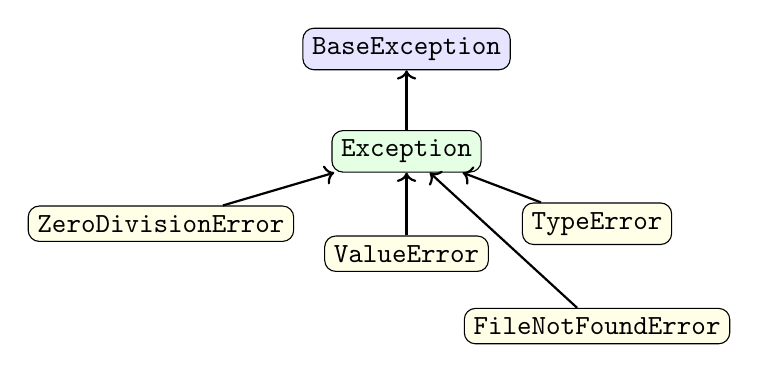
\begin{tikzpicture}[node distance=1.3cm, every node/.style={font=\ttfamily}]
\node (base) [draw, rounded corners, fill=blue!10] {BaseException};
\node (exc) [below of=base, draw, rounded corners, fill=green!10] {Exception};
\node (zero) [below left of=exc, xshift=-2.2cm, draw, rounded corners, fill=yellow!10] {ZeroDivisionError};
\node (value) [below of=exc, draw, rounded corners, fill=yellow!10] {ValueError};
\node (type) [below right of=exc, xshift=1.5cm, draw, rounded corners, fill=yellow!10] {TypeError};
\node (file) [below right of=value, xshift=1.5cm, draw, rounded corners, fill=yellow!10] {FileNotFoundError};

\draw[->, thick] (exc) -- (base);
\draw[->, thick] (zero) -- (exc);
\draw[->, thick] (value) -- (exc);
\draw[->, thick] (type) -- (exc);
\draw[->, thick] (file) -- (exc);
\end{tikzpicture}

\vspace{10pt}
{\small Semua exception di Python diturunkan dari \texttt{BaseException}.}
\end{frame}

\begin{frame}[fragile]{Hierarki Exception di Python}
\vspace*{20pt}
\begin{itemize}
  \item Semua exception di Python berasal dari \texttt{BaseException}.
  \item Sebagian besar exception umum diturunkan dari \texttt{Exception}.
  \item Menangkap \texttt{Exception} berarti menangkap semua turunannya.
\end{itemize}

\begin{lstlisting}[style=PythonStyle]
try:
    x = int("abc")  # menyebabkan ValueError
except Exception as e:
    print("Terjadi kesalahan:", e)
\end{lstlisting}

\begin{lstlisting}[language=bash]
Terjadi kesalahan: invalid literal for int() with base 10: 'abc'
\end{lstlisting}
\end{frame}

\begin{frame}[fragile]{\texttt{as} untuk Mendapatkan Objek Exception}
\vspace*{10pt}
\begin{columns}[T,totalwidth=\textwidth]
\begin{column}{0.55\textwidth}
\begin{itemize}
  \item Kata kunci \texttt{as} menangkap objek exception ke variabel.
  \item Objek ini menyimpan detail seperti:
  \begin{itemize}
    \item Jenis kesalahan (\texttt{type(e).__name__})
    \item Pesan kesalahan (\texttt{e})
  \end{itemize}
\end{itemize}

\begin{lstlisting}[style=PythonStyle]
try:
    angka = int(input("Masukkan angka: "))
    hasil = 100 / angka
    print("Hasil:", hasil)
except Exception as e:
    print("Tipe kesalahan:", type(e).__name__)
    print("Pesan kesalahan:", e)
\end{lstlisting}
\end{column}

\begin{column}{0.4\textwidth}
\begin{lstlisting}[language=bash]
Masukkan angka: 0
Tipe kesalahan: ZeroDivisionError
Pesan kesalahan: division by zero

Masukkan angka: abc
Tipe kesalahan: ValueError
Pesan kesalahan: invalid literal
\end{lstlisting}

\begin{itemize}
  \item Dapat digunakan untuk mencatat log error.
  \item Membantu debugging lebih efisien.
\end{itemize}
\end{column}
\end{columns}
\end{frame}


\section{Blok Else dan Finally}

% ----------------------------------------------------------
\subsection*{Blok Else}
\begin{frame}[fragile]{Blok Else}
\vspace*{10pt}
\begin{columns}[T]
\begin{column}{0.6\textwidth}
\begin{itemize}
  \item Blok \texttt{else} dijalankan hanya jika tidak terjadi exception.
  \item Memisahkan logika utama dari penanganan error.
\end{itemize}

\begin{lstlisting}[style=PythonStyle]
try:
    angka = int(input("Masukkan angka: "))
    hasil = 100 / angka
except ZeroDivisionError:
    print("Error: Pembagian nol.")
except ValueError:
    print("Error: Input bukan angka.")
else:
    print("Hasil perhitungan:", hasil)
\end{lstlisting}
\end{column}

\begin{column}{0.35\textwidth}
\begin{lstlisting}[language=bash]
Masukkan angka: 5
Hasil perhitungan: 20.0

Masukkan angka: 0
Error: Pembagian nol.
\end{lstlisting}

\begin{itemize}
  \item Kode dalam \texttt{else} hanya berjalan jika \texttt{try} berhasil.
  \item Struktur lebih bersih dan mudah dibaca.
\end{itemize}
\end{column}
\end{columns}
\end{frame}

% ----------------------------------------------------------
\subsection*{Blok Finally}
\begin{frame}[fragile]{Blok Finally}
\vspace*{10pt}
\begin{columns}[T]
\begin{column}{0.6\textwidth}
\begin{itemize}
  \item Blok \texttt{finally} selalu dijalankan,
  baik ada error maupun tidak.
  \item Umumnya digunakan untuk \textit{cleanup} seperti menutup file.
\end{itemize}

\begin{lstlisting}[style=PythonStyle]
f = None
try:
    f = open("data.txt", "r")
    isi = f.read()
    print("Isi file:", isi)
except FileNotFoundError:
    print("Error: File tidak ditemukan.")
finally:
    if f is not None:
        f.close()
        print("File berhasil ditutup.")
\end{lstlisting}
\end{column}

\begin{column}{0.35\textwidth}
\begin{lstlisting}[language=bash]
Error: File tidak ditemukan.

Isi file: Halo dunia!
File berhasil ditutup.
\end{lstlisting}

\begin{itemize}
  \item \texttt{finally} memastikan tindakan penting tetap dilakukan.
  \item Cocok untuk menutup file, koneksi, atau membersihkan memori.
\end{itemize}
\end{column}
\end{columns}
\end{frame}

\begin{frame}{Diagram Alur Try-Except-Else-Finally}
\vspace*{10pt}
\begin{columns}[T,totalwidth=\textwidth]
% Left column: diagram
\begin{column}{0.58\textwidth}
\centering
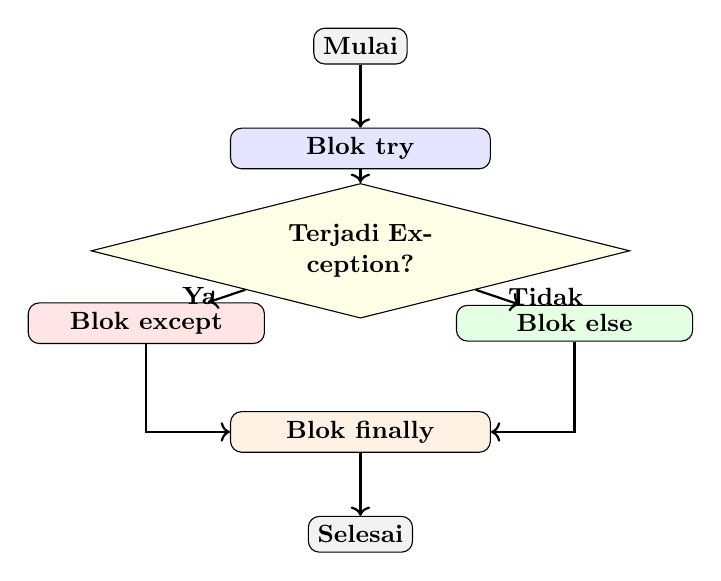
\begin{tikzpicture}[node distance=1.3cm, font=\small, align=center]
\node (start) [draw, rounded corners, fill=gray!10] {\textbf{Mulai}};
\node (try) [below of=start, draw, rounded corners, fill=blue!10, minimum width=3.3cm] {\textbf{Blok try}};
\node (error?) [below of=try, draw, diamond, aspect=4, fill=yellow!10, text width=3cm] {\textbf{Terjadi Exception?}};
\node (except) [below left of=error?, xshift=-1.8cm, draw, rounded corners, fill=red!10, minimum width=3cm] {\textbf{Blok except}};
\node (else) [below right of=error?, xshift=1.8cm, draw, rounded corners, fill=green!10, minimum width=3cm] {\textbf{Blok else}};
\node (finally) [below of=error?, yshift=-1cm, draw, rounded corners, fill=orange!10, minimum width=3.3cm] {\textbf{Blok finally}};
\node (end) [below of=finally, draw, rounded corners, fill=gray!10] {\textbf{Selesai}};

\draw[->, thick] (start) -- (try);
\draw[->, thick] (try) -- (error?);
\draw[->, thick] (error?) -- node[left]{\textbf{Ya}} (except);
\draw[->, thick] (error?) -- node[right]{\textbf{Tidak}} (else);
\draw[->, thick] (except) |- (finally);
\draw[->, thick] (else) |- (finally);
\draw[->, thick] (finally) -- (end);
\end{tikzpicture}
\end{column}

% Right column: explanation
\begin{column}{0.37\textwidth}
\small
\begin{itemize}
  \item \textbf{Blok try} – berisi kode utama yang berisiko error.
  \item \textbf{Blok except} – menangani kesalahan yang terjadi.
  \item \textbf{Blok else} – dijalankan jika tidak ada error.
  \item \textbf{Blok finally} – selalu dijalankan, baik ada error maupun tidak.
\end{itemize}

\vspace{6pt}
\textit{Struktur ini memastikan program tetap stabil dan semua proses penting diselesaikan dengan aman.}
\end{column}
\end{columns}
\end{frame}

\section{Membuat Exception Sendiri}

% ----------------------------------------------------------
\subsection*{Pengenalan Custom Exception}
\begin{frame}[fragile]{Pengenalan Custom Exception}
\vspace*{10pt}
\begin{columns}[T,totalwidth=\textwidth]
\begin{column}{0.58\textwidth}
\begin{itemize}
  \item \textbf{Custom exception} memungkinkan kita membuat tipe kesalahan sendiri.
  \item Berguna untuk konteks aplikasi tertentu, misalnya:
  \begin{itemize}
    \item \texttt{SaldoTidakCukupError}
    \item \texttt{TransaksiTidakValidError}
  \end{itemize}
  \item Membuat kode lebih bermakna dan mudah dibaca.
\end{itemize}
\end{column}

\begin{column}{0.37\textwidth}
\begin{block}{\textbf{Contoh Kasus}}
\small
Dalam aplikasi keuangan:
\begin{itemize}
  \item Menolak transaksi di bawah saldo minimum.
  \item Menandai data transaksi tidak valid.
\end{itemize}
\textit{Custom exception memperjelas jenis kesalahan yang terjadi.}
\end{block}
\end{column}
\end{columns}
\end{frame}

% ----------------------------------------------------------
\subsection*{Cara Mendefinisikan Class Exception Sendiri}
\begin{frame}[fragile]{Cara Mendefinisikan Class Exception Sendiri}
\vspace*{10pt}
\begin{columns}
\begin{column}[t]{0.60\textwidth}
\begin{lstlisting}[style=PythonStyle, basicstyle=\ttfamily\scriptsize]
class InputNegatifError(Exception):
    """Exception jika input bernilai negatif."""
    pass

def hitung_akar(x):
    if x < 0:
        raise InputNegatifError(
            "Tidak bisa menghitung akar dari bilangan negatif!"
        )
    return x ** 0.5

try:
    angka = int(input("Masukkan angka: "))
    print("Hasil akar:", hitung_akar(angka))
except InputNegatifError as e:
    print("Terjadi kesalahan:", e)
\end{lstlisting}
\end{column}

\begin{column}[t]{0.35\textwidth}
\begin{lstlisting}[language=bash]
Masukkan angka: -9
Terjadi kesalahan: 
Tidak bisa menghitung akar dari 
bilangan negatif!
\end{lstlisting}

\begin{itemize}
  \item Gunakan \texttt{raise} untuk melempar exception.
  \item Cocok untuk validasi logika domain.
\end{itemize}
\end{column}
\end{columns}
\end{frame}

% ----------------------------------------------------------
\subsection*{Atribut dan Konstruktor Khusus}
\begin{frame}[fragile]{Atribut dan Konstruktor Khusus}
\vspace*{10pt}
\begin{columns}
\begin{column}[t]{0.60\textwidth}
\begin{lstlisting}[style=PythonStyle, basicstyle=\ttfamily\scriptsize]
class NilaiTidakValidError(Exception):
    """Exception untuk nilai di luar rentang."""
    def __init__(self, nilai, pesan="Nilai di luar rentang."):
        self.nilai = nilai
        self.pesan = pesan
        super().__init__(self.pesan)

def set_nilai(nilai):
    if nilai < 0 or nilai > 100:
        raise NilaiTidakValidError(nilai)
    print(f"Nilai {nilai} disimpan sukses.")

try:
    set_nilai(150)
except NilaiTidakValidError as e:
    print(f"Error: {e.pesan} (nilai: {e.nilai})")
\end{lstlisting}
\end{column}

\begin{column}[t]{0.35\textwidth}
\begin{lstlisting}[language=bash]
Error: Nilai di luar rentang.
(nilai: 150)
\end{lstlisting}

\begin{itemize}
  \item Tambahkan atribut untuk informasi kontekstual.
  \item Memudahkan pelacakan dan debugging.
\end{itemize}
\end{column}
\end{columns}
\end{frame}

% ----------------------------------------------------------
\begin{frame}[fragile]{Studi Kasus: Validasi Input Pengguna (1/2)}
\vspace*{10pt}
\begin{columns}[T,totalwidth=\textwidth]
\begin{column}{0.60\textwidth}
\begin{lstlisting}[style=PythonStyle, basicstyle=\ttfamily\scriptsize]
class UsiaTidakValidError(Exception):
    """Exception untuk usia tidak logis."""
    def __init__(self, usia, pesan="Usia tidak valid."):
        self.usia = usia
        self.pesan = pesan
        super().__init__(self.pesan)

def input_usia():
    usia = int(input("Masukkan usia Anda: "))
    if usia < 0:
        raise UsiaTidakValidError(usia, "Usia tidak boleh negatif.")
    elif usia > 120:
        raise UsiaTidakValidError(usia, "Usia terlalu besar.")
    return usia
\end{lstlisting}
\end{column}

\begin{column}{0.35\textwidth}
\small
\textbf{Penjelasan:}
\begin{itemize}
  \item \texttt{UsiaTidakValidError} adalah \textbf{custom exception}.
  \item Digunakan untuk memvalidasi input agar masuk akal.
  \item \texttt{raise} melempar kesalahan ketika data tidak valid.
  \item Pemisahan logika validasi membuat kode lebih bersih.
\end{itemize}
\end{column}
\end{columns}
\end{frame}


% ----------------------------------------------------------
\begin{frame}[fragile]{Studi Kasus: Validasi Input Pengguna (2/2)}
\vspace*{10pt}
\begin{columns}[T,totalwidth=\textwidth]
\begin{column}{0.60\textwidth}
\begin{lstlisting}[style=PythonStyle, basicstyle=\ttfamily\scriptsize]
try:
    umur = input_usia()
    print("Usia Anda adalah:", umur)
except UsiaTidakValidError as e:
    print(f"Error: {e.pesan} (diberikan: {e.usia})")
except ValueError:
    print("Error: Input harus berupa angka.")
\end{lstlisting}

\begin{itemize}
  \item \texttt{try-except} menangani dua jenis kesalahan:
  \begin{itemize}
    \item \texttt{UsiaTidakValidError} – logika usia tidak valid.
    \item \texttt{ValueError} – input bukan angka.
  \end{itemize}
  \item Mencegah program berhenti tiba-tiba dan memberikan umpan balik jelas.
\end{itemize}
\end{column}

\begin{column}{0.35\textwidth}
\begin{lstlisting}[language=bash, basicstyle=\ttfamily\scriptsize]
Masukkan usia Anda: -5
Error: Usia tidak boleh negatif.
(diberikan: -5)

Masukkan usia Anda: 130
Error: Usia terlalu besar.
(diberikan: 130)

Masukkan usia Anda: 25
Usia Anda adalah: 25
\end{lstlisting}


\textbf{Custom exception} membuat pesan kesalahan lebih kontekstual.
Menjaga validasi input tetap jelas, aman, dan mudah dipelihara.

\end{column}
\end{columns}
\end{frame}


\begin{frame}{Rangkuman}
\vspace*{15pt}
\begin{itemize}
  \item Kesalahan (\textit{error}) adalah bagian alami dari pemrograman dan ditangani melalui mekanisme \textbf{exception}.
  \item Python membedakan antara \textbf{syntax error} (saat kompilasi) dan \textbf{runtime error}/\textit{exception} (saat eksekusi).
  \item Dengan \texttt{try-except}, program tidak perlu berhenti tiba-tiba; kita dapat menampilkan pesan ramah atau memperbaiki kesalahan.
  \item Gunakan \texttt{else} untuk eksekusi normal dan \texttt{finally} untuk pembersihan.
  \item \textbf{Custom exception} membantu mendefinisikan kesalahan sesuai konteks aplikasi.
  \item Pemahaman ini menjadi dasar penting sebelum mempelajari \textbf{unit testing} guna menjaga keandalan program.
\end{itemize}
\end{frame}





\end{document}